\section{Desarrollo}

\subsection{Dependencias y uso del código adjunto}

Las herramientas utilizadas para realizar la experimentación de este trabajo se encuentran adjuntas y son scripts en Python. Las dependencias necesarias para poder correr todos los scripts son:

\begin{itemize}
  \item Requests
  \item Numpy
  \item Scapy
  \item MatPlotLib
\end{itemize}

El modo de uso es para el ejercicio de Traceroute (3.1):

\begin{verbatim}
$ sudo python traceroute.py <URL>
\end{verbatim}

También se puede llamar al Traceroute junto con la geolocalización y la imagen del mapa utilizando esta forma (ejercicio 3.2):

\begin{verbatim}
$ sudo python plot.py <URL>
\end{verbatim}

Por último, para ejecutar el script que realiza el Ping (ejercicio 3.3):

\begin{verbatim}
$ sudo python ping.py <URL>
\end{verbatim}

\subsection{Ejercicio 3.1: Caracterizando rutas}

% Descripción del algoritmo
El Traceroute envía tres paquetes ICMP Echo Request por cada TTL. Comienza
con un $TTL_0$ inicial de 1 y lo incrementa de esta forma: $TTL_{i+1} = TTL_i + 1$,
hasta que el mismo llega a 30 o se recibe una respuesta ICMP Echo Reply
del nodo destino. Cada router o hop decrementa en 1 el valor del TTL o hop limit y si
el mismo llega a 0 responde al origen con un paquete ICMP Time Exceeded. De esta forma,
podemos conocer todos los hops intermedios que atraviesa un paquete para llegar al destino
elegido inspeccionando las respuestas recibidas para cada TTL.
En los casos en los que contábamos con más
de una IP para un determinado TTL \textit{(es decir, nos respondían diferentes hops)} tomamos la que apareció más veces o, de no existir
una que cumpla con ese criterio, la que obtuvimos primero.\\
\par
% Definición del scope
El objetivo del traceroute es conocer una de las rutas posibles hasta el nodo destino.
Nuestra implementación envía sólo tres paquetes
por TTL, como el traceroute que se encuentra en los sistemas operativos más populares,
porque como no se tiene ningún control sobre la ruta que los paquetes toman no podemos
asegurar que enviando una mayor cantidad de paquetes obtengamos resultados más fieles.
Incluso puede ser que los hops intermedios obtenidos no pertenezcan a una misma ruta
ya que quizás cuando se envió el paquete con $TTL_2$ no se pasó por el mismo router que
se alcanzó cuando se envió el paquete con el $TTL_1$.\\
\par
% Posibles problemas
Cuando ejecutamos el traceroute con ciertos destinos, por ejemplo \textit{dc.uba.ar},
 el TTL crecía indefinidamente y nunca obteníamos un Echo Reply de nuestro destino.
Por esta razón creimos conveniente imponer un límite a la cantidad de hops permitidas.
Nos inclinamos por 30 para seguir la tradición de los traceroute de Unix.\\
\par

El output que se obtiene al ejecutar nuestro Traceroute tiene el siguiente formato:

\begin{table}[H]
    \begin{tabular}{lllll}
     TTL &  RTT     &  ZRTT         &   \%Resp       &  HOP            \\
    1    & 17.89    &  -0.68        &  100.0         &  10.2.203.254   \\
    2    & 12.35    &  -0.70        &  100.0         &  157.92.18.99   \\
    3    & 0.00     &  -0.76        &  0.0           &  *              \\
    4    & 12.56    &  -0.70        &  100.0         &  157.92.47.98   \\
    \end{tabular}
\end{table}

El RTT es el promedio obtenido de los RTT de los tres paquetes enviados y el ZRTT es
calculado a partir del promedio general $\overline{RTT}$ y del SRTT:
\begin{displaymath}
  \overline{RTT} = \frac{\sum_{i = 1}^{n} RTT_i}{n}
\end{displaymath}
donde $n$ es la cantidad de hops hasta el nodo destino y $RTT_i$ el promedio de los
RTTs de los tres paquetes enviados con $TTL = i$, el mismo que aparece en el output
de la herramienta. El SRTT es el desvío estándard de los RTT de la ruta:
\begin{displaymath}
  SRTT = \sqrt[2]{\frac{\sum_{i = 1}^{n} (RTT_i-\overline{RTT})^2}{n}}
\end{displaymath}
contando con el $\overline{RTT}$ y el SRTT podemos obtener el ZRTT mediante la siguiente
fórmula:
\begin{displaymath}
  ZRTT_i = \frac{RTT_i - \overline{RTT}}{SRTT}
\end{displaymath}

A continuación presentamos las tablas obtenidas para las 4 universidades elegidas.
Realizaremos nuestro análisis a partir de éstas y los gráficos de la sección subsiguiente,
éste lo concentraremos en el apartado de \textbf{Discusión}.

\subsubsection{Universidad Católica de Australia (ACU)}

\begin{table}[H]
    \begin{tabular}{lllll}
    TTL & RTT    & ZRTT  & \%Resp & HOP             \\
    1   & 89.53  & -0.47 & 100.0  & 192.168.0.1     \\
    2   & 87.93  & -0.47 & 100.0  & 10.24.128.1     \\
    3   & 87.88  & -0.47 & 100.0  & 181.47.254.85   \\
    4   & 101.28 & -0.42 & 100.0  & 208.178.195.214 \\
    5   & 90.54  & -0.46 & 100.0  & 208.178.195.213 \\
    6   & 221.26 & 0.04  & 100.0  & 67.16.139.18    \\
    7   & 207.92 & -0.01 & 100.0  & 64.212.107.98   \\
    8   & 210.58 & -0.00 & 100.0  & 129.250.3.172   \\
    9   & 0.00   & -0.81 & 0.0    & *               \\
    10  & 239.94 & 0.11  & 100.0  & 129.250.2.59    \\
    11  & 269.25 & 0.22  & 100.0  & 129.250.4.154   \\
    12  & 257.23 & 0.18  & 100.0  & 129.250.4.24    \\
    13  & 281.28 & 0.27  & 100.0  & 128.241.219.154 \\
    14  & 425.20 & 0.82  & 100.0  & 202.158.194.161 \\
    15  & 403.03 & 0.73  & 100.0  & 113.197.15.65   \\
    16  & 423.50 & 0.81  & 100.0  & 202.158.194.241 \\
    17  & 417.22 & 0.79  & 100.0  & 202.158.207.226 \\
    18  & 421.26 & 0.80  & 100.0  & 202.158.207.230 \\
    19  & 0.00   & -0.81 & 0.0    & *               \\
    20  & 0.00   & -0.81 & 0.0    & *               \\
    21  & 418.61 & 0.79  & 100.0  & 192.148.223.248 \\
    \end{tabular}
    \caption{Resultado del traceroute para Australia}
  \label{fig:tabla-aus}
\end{table}

\subsubsection{Universidad of Bergen (UIB) - Noruega}

\begin{table}[H]
    \begin{tabular}{lllll}
     TTL &  RTT     &  ZRTT         &   \%Resp       &  HOP            \\
    1    & 17.89    &  -0.68        &  100.0         &  10.2.203.254   \\
    2    & 12.35    &  -0.70        &  100.0         &  157.92.18.99   \\
    3    & 0.00     &  -0.76        &  0.0           &  *              \\
    4    & 12.56    &  -0.70        &  100.0         &  157.92.47.98   \\
    5    & 11.53    &  -0.70        &  100.0         &  157.92.47.2    \\
    6    & 0.00     &  -0.76        &  0.0           &  *              \\
    7    & 102.99   &   -0.27       &  100.0         &  168.96.0.18    \\
    8    & 58.54    &  -0.48        &  100.0         &  200.0.204.154  \\
    9    & 123.07   &   -0.18       &  100.0         &  200.0.204.63   \\
    10   &   284.44 &   0.58        &   100.0        &  62.40.124.36   \\
    11   &   273.62 &   0.53        &   100.0        &  62.40.124.130  \\
    12   &   337.27 &   0.83        &   100.0        &  109.105.97.126 \\
    13   &   334.97 &   0.82        &   100.0        &  109.105.102.26 \\
    14   &   282.40 &   0.57        &   100.0        &  128.39.231.66  \\
    15   &   307.80 &   0.69        &   66.7         &  128.39.254.193 \\
    16   &   319.86 &   0.75        &   100.0        &  158.37.1.190   \\
    17   &   274.32 &   0.53        &   100.0        &  129.177.1.122  \\
    18   &   313.06 &   0.71        &   100.0        &  129.177.6.99   \\
    \end{tabular}
    \caption{Resultado del traceroute para Noruega}
  \label{fig:tabla-nor}
\end{table}

\subsubsection{Universidad de Tokyo - Japón}

\begin{table}[H]
    \begin{tabular}{lllll}
    TTL & RTT    & ZRTT  & \%Resp & HOP             \\
    1   & 114.83 & -0.48 & 100.0  & 192.168.0.1     \\
    2   & 95.85  & -0.54 & 100.0  & 10.24.128.1     \\
    3   & 78.51  & -0.61 & 100.0  & 181.47.254.85   \\
    4   & 91.94  & -0.56 & 100.0  & 208.178.195.214 \\
    5   & 102.53 & -0.52 & 100.0  & 208.178.195.213 \\
    6   & 219.92 & -0.10 & 100.0  & 67.16.139.18    \\
    7   & 223.94 & -0.09 & 100.0  & 129.250.9.117   \\
    8   & 229.24 & -0.07 & 100.0  & 129.250.3.172   \\
    9   & 235.85 & -0.05 & 33.3   & 129.250.2.219   \\
    10  & 252.05 & 0.01  & 66.7   & 129.250.7.69    \\
    11  & 377.22 & 0.46  & 100.0  & 129.250.4.39    \\
    12  & 395.96 & 0.52  & 100.0  & 129.250.6.90    \\
    13  & 373.15 & 0.44  & 100.0  & 61.200.80.218   \\
    14  & 382.62 & 0.48  & 100.0  & 158.205.192.173 \\
    15  & 393.17 & 0.51  & 100.0  & 158.205.192.86  \\
    16  & 394.56 & 0.52  & 100.0  & 158.205.121.250 \\
    17  & 383.91 & 0.48  & 100.0  & 154.34.240.254  \\
    18  & 381.23 & 0.47  & 100.0  & 210.152.135.178 \\
    \end{tabular}
    \caption{Resultado del traceroute para Japón}
  \label{fig:tabla-tok}
\end{table}

\subsubsection{Lomonosov Universidad del estado de Moscú - Rusia}

\begin{table}[H]
  \begin{tabular}{lllll}
     TTL &  RTT      &  ZRTT   &   \%Resp &  HOP              \\
    1  	 &  47,51	   &  0,53	 &   100	  &  181.170.214.1 (Argentina)        \\
    2  	 &  0	       &  0,75	 &   0	    &  * (Desconocido)                  \\
    3  	 &  0	       &  0,75	 &   0	    &  * (Desconocido)                  \\
    4  	 &  0	       &  0,75	 &   0	    &  * (Desconocido)                  \\
    5  	 &  43,75	   &  0,55	 &   66,7	  &  200.89.166.209 (Argentina)       \\
    6  	 &  46,22	   &  0,54	 &   100	  &  200.89.165.222 (Argentina)       \\
    7  	 &  51,06	   &  0,52	 &   100	  &  207.136.166.241 (United States)  \\
    8  	 &  178,22	 &  0,07	 &   100	  &  67.17.68.234 (United States)     \\
    9  	 &  172,53	 &  0,04	 &   100	  &  4.68.111.121 (United States)     \\
    10	 &  288,12	 &  0,58	 &   100	  &  4.69.158.245 (United States)     \\
    11	 &  297,24	 &  0,62	 &   66,7	  &  4.69.158.245 (United States)     \\
    12	 &  326,95	 &  0,76	 &   100	  &  213.242.110.198 (United States)  \\
    13	 &  0	       &  0,75	 &   0	    &  * (Desconocido)                  \\
    14	 &  328,28	 &  0,76	 &   100	  &  194.85.40.229 (Russia)           \\
    15	 &  327,94	 &  0,76	 &   100	  &  194.190.254.118 (Russia)         \\
    16	 &  341,56	 &  0,82	 &   66,7	  &  93.180.0.174 (Russia)            \\
    17	 &  324,37	 &  0,74	 &   100	  &  188.44.33.1 (Russia)             \\
    18	 &  327,28	 &  0,76	 &   100	  &  188.44.50.103 (Russia)           \\
    \end{tabular}
    \caption{Resultado del traceroute para Rusia}
  \label{fig:tabla-rus}
\end{table}

\newpage

\subsection{Ejercicio 3.2: Gráficos y análisis}
% Descripción de la sección
Implementamos una herramienta que permite geolocalizar una secuencia de IPs y unirlas
en el orden recibido. La utilizamos para mostrar las rutas que obtuvimos del
traceroute sobre un mapa y que así se pueda apreciar más fácilmente el camino
recorrido a través de los distintos hops.\\
\par
% Cómo se realizó la geolocalización
La geolocalización de las IPs se realizó consultando a la API que provee \textit{https://freegeoip.net}.
Los productos que ofrecen este tipo de servicios utilizan bases de datos que mapean
rangos de IPs a zonas geográficas o ISPs particulares. El mapeo se basa principalmente
en la información obtenida de los registros regionales de internet:
\begin{itemize}
  \item African Network Information Centre (AfriNIC)
  \item American Registry for Internet Numbers (ARIN)
  \item Asia-Pacific Network Information Centre (APNIC)
  \item Latin American and Caribbean Internet Address Registry (LACNIC)
  \item RIPE Network Coordination Centre (RIPE NCC)
\end{itemize}
que son los entes que regulan la asignación de IPs por región.\\
\par
% Desventajas de la geolocalización por IP
Las consultas devuelven una latitud y una longitud específica, sin embargo, éstas no
corresponden con la ubicación precisa del dispositivo que porta esa IP sino con la
ubicación del organismo o el ISP que asignó esa IP. La precisión de la geolocalización 
dependerá de la base de datos con la cual se realice el mapeo. Por esa razón en los mapas
se ven una cantidad de hops mucho menor a la que presenta el traceroute, varios hops son
geolocalizados a la misma ubicación.\\
\par
% Descripción de los gráficos estadísticos
Además, elaboramos gráficos para reflejar el comportamiento del RTT y el ZRTT a lo
largo de las rutas realizadas. Esperamos con ellos poder identificar movimientos
significativos que nos indiquen la presencia de enlaces submarinos entre determinados
hops.
Todos los gráficos están ordenados por TTL crecientemente, pero para poder dar más
contexto elegimos precisar en el eje Y el hop y no el orden de TTL.

\subsubsection{Universidad Católica de Australia (ACU)}

\begin{figure}[H]
  \centering
    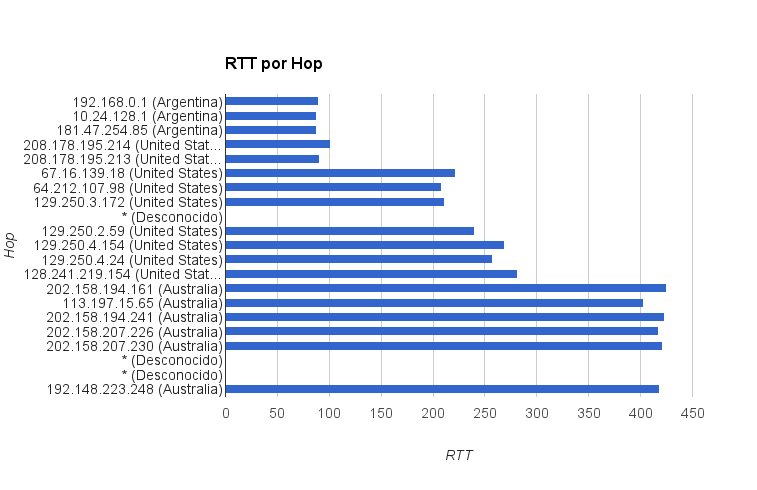
\includegraphics[width=1\textwidth]{../Experimentacion/Australia/rtt.png}
    \caption{RTT por IP para Australia}
  \label{rtt-aus}
\end{figure}

\begin{figure}[H]
  \centering
    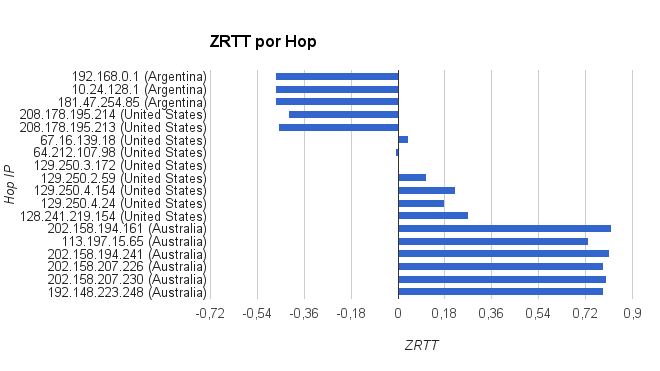
\includegraphics[width=1\textwidth]{../Experimentacion/Australia/zrtt.png}
    \caption{ZRTT por IP para Australia}
  \label{zrtt-aus}
\end{figure}

\begin{figure}[H]
  \centering
    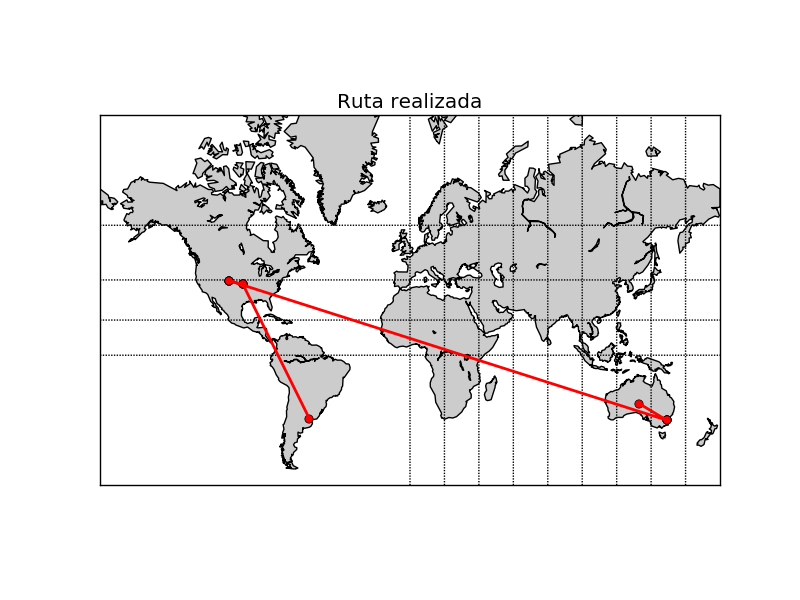
\includegraphics[width=1\textwidth]{../Experimentacion/Australia/map.png}
    \caption{Mapa de ruta para Australia}
  \label{map-aus}
\end{figure}

\subsubsection{Universidad of Bergen (UIB) - Noruega}

\begin{figure}[H]
  \centering
    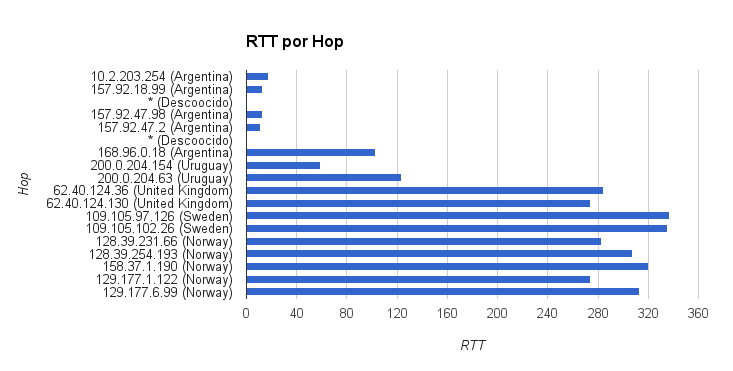
\includegraphics[width=1\textwidth]{../Experimentacion/Noruega/rtt.png}
    \caption{RTT por IP para Noruega}
  \label{rtt-nor}
\end{figure}

\begin{figure}[H]
  \centering
    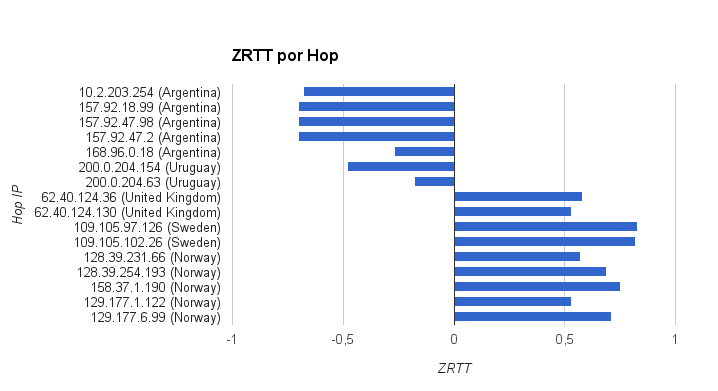
\includegraphics[width=1\textwidth]{../Experimentacion/Noruega/zrtt.png}
    \caption{ZRTT por IP para Noruega}
  \label{zrtt-nor}
\end{figure}

\begin{figure}[H]
  \centering
    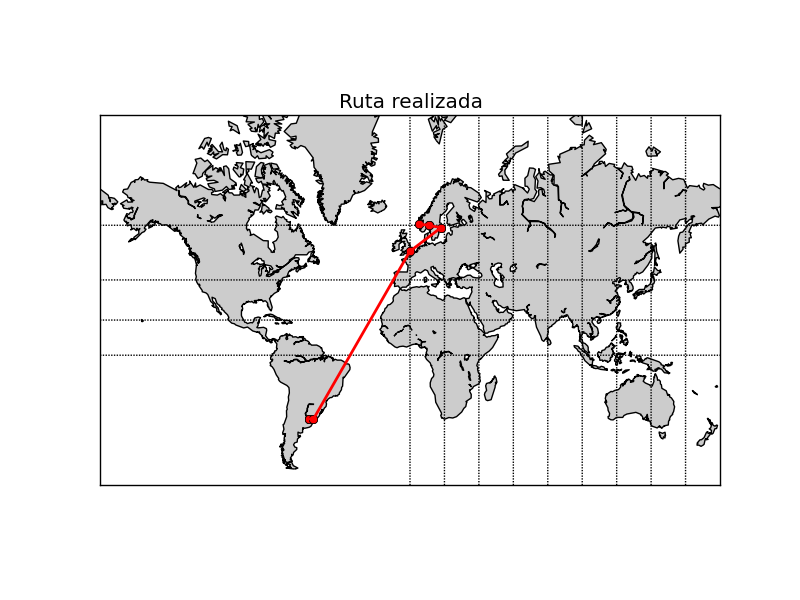
\includegraphics[width=1\textwidth]{../Experimentacion/Noruega/map.png}
    \caption{Mapa de ruta para Noruega}
  \label{map-nor}
\end{figure}

\subsubsection{Universidad de Tokyo - Japón}

\begin{figure}[H]
  \centering
    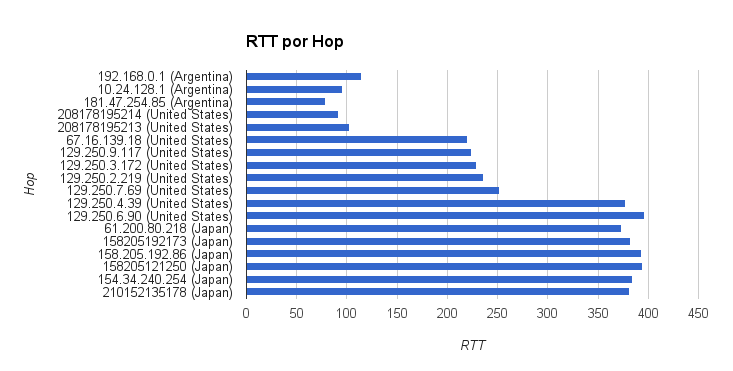
\includegraphics[width=1\textwidth]{../Experimentacion/Tokyo/rtt.png}
    \caption{RTT por IP para Japón}
  \label{rtt-tok}
\end{figure}

\begin{figure}[H]
  \centering
    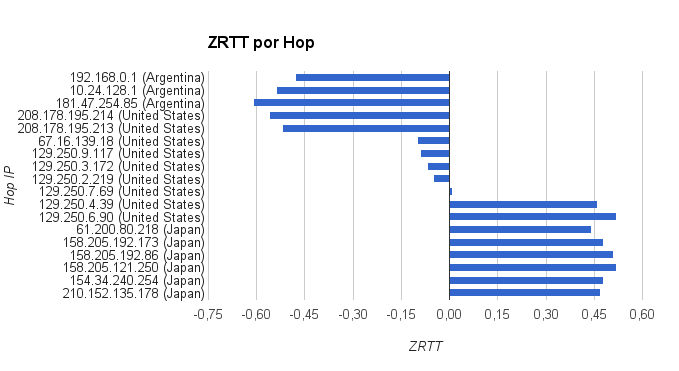
\includegraphics[width=1\textwidth]{../Experimentacion/Tokyo/zrtt.png}
    \caption{ZRTT por IP para Japón}
  \label{zrtt-tok}
\end{figure}

\begin{figure}[H]
  \centering
    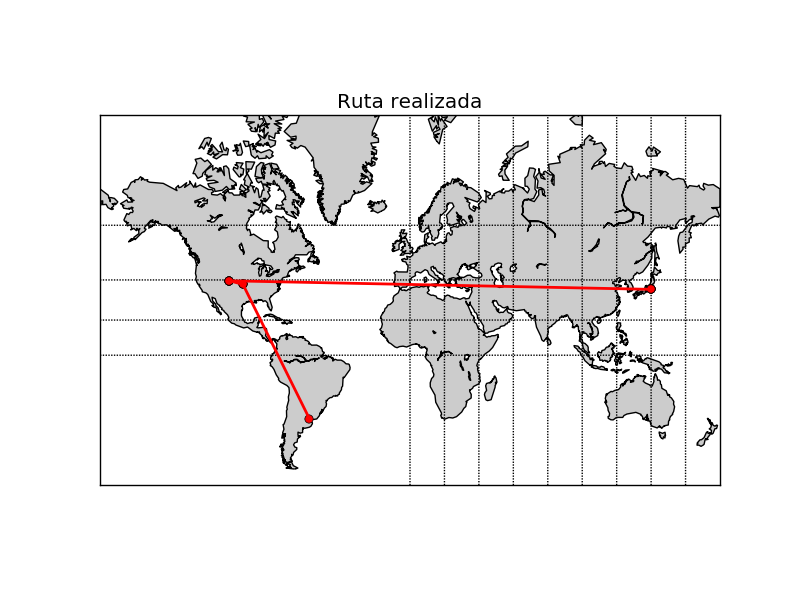
\includegraphics[width=1\textwidth]{../Experimentacion/Tokyo/map.png}
    \caption{Mapa de ruta para Japón}
  \label{map-tok}
\end{figure}

\subsubsection{Lomonosov Universidad del estado de Moscú - Rusia}

\begin{figure}[H]
  \centering
    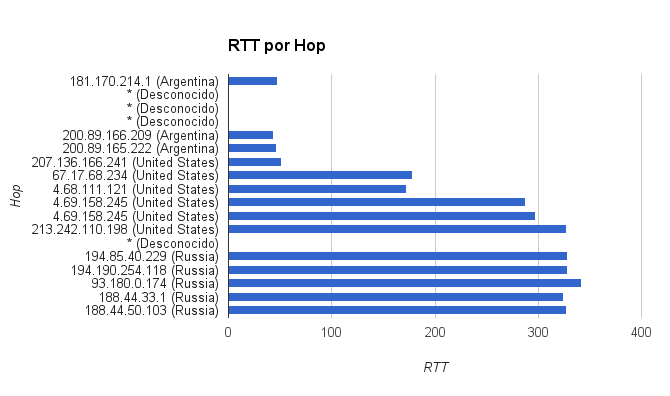
\includegraphics[width=1\textwidth]{../Experimentacion/Rusia/rtt.png}
    \caption{RTT por IP para Rusia}
  \label{rtt-rus}
\end{figure}

\begin{figure}[H]
  \centering
    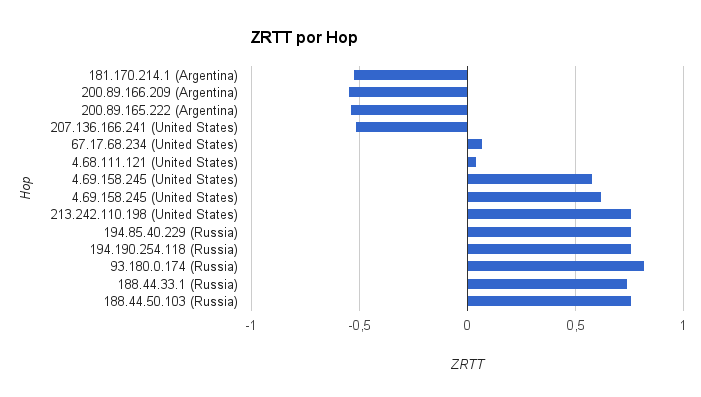
\includegraphics[width=1\textwidth]{../Experimentacion/Rusia/zrtt.png}
    \caption{ZRTT por IP para Rusia }
  \label{zrtt-rus}
\end{figure}

\begin{figure}[H]
  \centering
    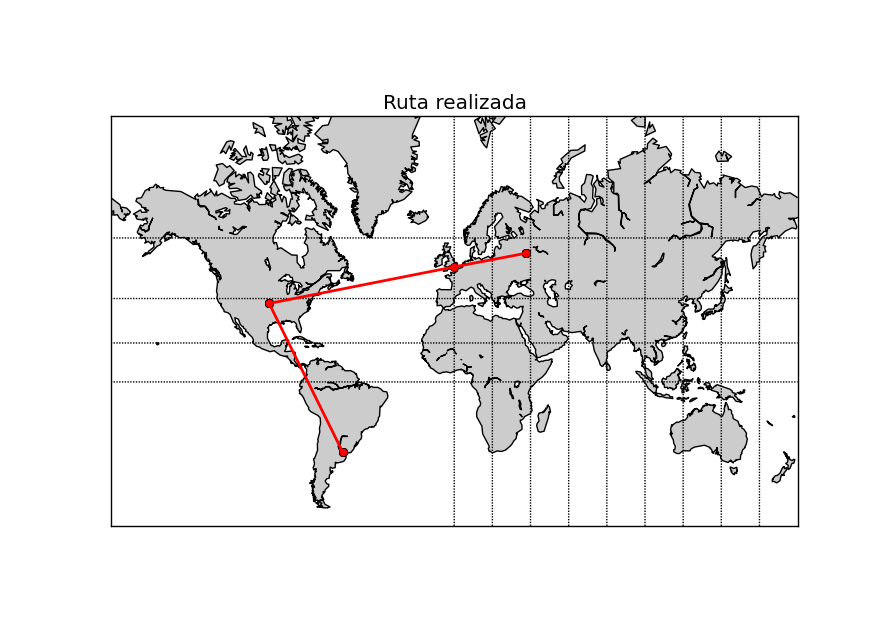
\includegraphics[width=1\textwidth]{../Experimentacion/Rusia/map.png}
    \caption{Mapa de ruta para Rusia}
  \label{map-rus}
\end{figure}

\newpage
\subsection{Ejercicio 3.3: Contrastando con la realidad}

En este punto queremos estimar mediante sucesivos pings el RTT existente entre el host origen \textit{(host desde el cual se realiza el ping)} y cada una de las cuatro universidades elegidas para este trabajo.
En cada ping enviamos un paquete ICMP Echo request y esperamos que el host destino nos responda con el correspondiente paquete ICMP Echo reply. Midiendo el tiempo transcurrido desde que enviamos el echo request hasta que recibimos el echo reply obtenemos una muestra $s_i$ del RTT entre los dos host. Luego, con dicha muestra aplicamos la siguiente fórmula para estimar con mayor fidelidad el RTT de la conexión:
\begin{center}
  $SRTT_{i+1}$ = ($\alpha$ * $SRTT_i$) + (1 - $\alpha$) * $s_i$
\end{center}

Tanto el valor de $\alpha$ como la cantidad de muestras $s_i$ obtenidas son valores que variamos.


Se puede ver que el valor de $\alpha$ controla cuán rápidamente el SRTT se adapta a cambios en la muestra de RTTs. Dado que siempre es posible que una respuesta en particular tarde mucho en llegar \textit{(ya sea por que tomo una ruta más larga que el resto de los paquetes, por un aumento momentáneo de la congestión en la red o por que el host destino retraso el envío de la respuesta)}, consideramos que valores de $\alpha$ por encima de $0.50$ implicarían, prácticamente, ignorar todos los valores muestreados anteriormente. Por este motivo, los valores elegidos para $\alpha$ fueron: $0.15$, $0.30$ y $0.50$.


Por otra parte, elegimos tres tamaños de muestra diferentes: $10$, $70$ y $150$.
Para cada una de las nueves combinaciones posibles entre tamaño de muestra y $\alpha$ estimamos la probabilidad de perdida de paquete como:
\begin{center}
	Probabilidad de perdida de paquetes estimada $=$ $1$ - $\frac{\#Echo\ reply}{\#Echo\ request}$
\end{center}

También calculamos el throughput de la conexión utilizando la fórmula para enlaces ideales, en los casos en que no hubo pérdida de paquetes:
\begin{displaymath}
  throughput = \frac{|Ventana|}{RTT}
\end{displaymath}

En esta fórmula fijamos el valor de $|Ventana|$ en 64 Kbytes.
En los casos en que sí hubo pérdida de paquetes, utilizamos la fórmula de Mathis:
\begin{center}
	throughput < $\frac{MSS}{RTT * \sqrt{p}}$
\end{center}

En dicha fórmula fijamos el valor de MSS \textit{Maximum Segment Size} en 1460 bytes.


A continuación mostraremos, para cada una de las cuatro universidades elegidas, los resultados de la experimentación realizada.

\subsubsection{Universidad Católica de Australia (ACU)}

\begin{figure}[H]
\begin{changemargin}{-5cm}{-5cm}
    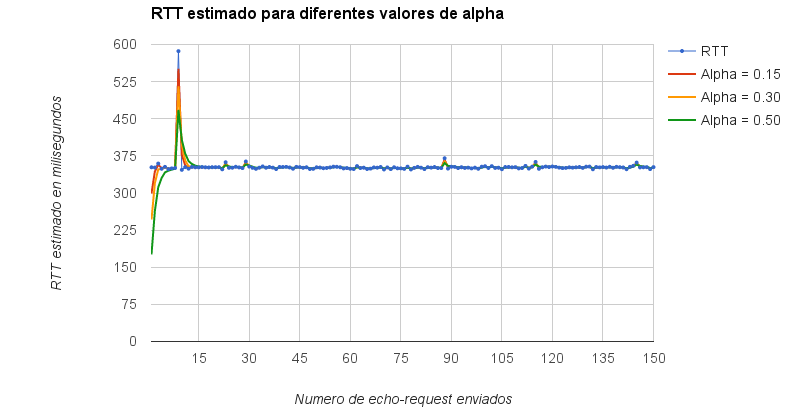
\includegraphics[width=1.5\textwidth]{../Experimentacion/Australia/ertt.png}
    \caption{RTT estimado por cada muestra de RTT para los diferentes valores de $\alpha$}
  \label{ertt-aus}
  \end{changemargin}
\end{figure}


\begin{table}[H]
	\centering
    \begin{tabular}{lllll}
    \hline
    \#Muestras & $\alpha$ & RTT estimado &Prob. estimada perdida paquete & Throughput \\	\hline
    10   &  0.15  &  351.79 ms  &  0.0\%  &  181.9 Kbyte/s  \\
    10   &  0.30  &  351.53 ms  &  0.0\%  &  182.0 Kbyte/s  \\
    10   &  0.50  &  350.73 ms  &  0.0\%  &  182.4 Kbyte/s  \\
    70   &  0.15  &  356.06 ms  &  0.0\%  &  179.7 Kbyte/s  \\
    70   &  0.30  &  354.87 ms  &  0.0\%  &  180.3 Kbyte/s  \\
    70   &  0.50  &  353.43 ms  &  0.0\%  &  181.0 Kbyte/s  \\
    150  &  0.15  &  351.75 ms  &  0.0\%  &  181.9 Kbyte/s  \\
    150  &  0.30  &  351.42 ms  &  0.0\%  &  182.1 Kbyte/s  \\
    150  &  0.50  &  351.38 ms  &  0.0\%  &  182.1 Kbyte/s  \\ \hline
    \end{tabular}
    \caption{Resultado del análisis de las muestras de RTTs para Australia}
  \label{fig:tabla-ertt-aus}
\end{table}


\subsubsection{Universidad de Bergen (UIB) - Noruega}

\begin{figure}[H]
\begin{changemargin}{-5cm}{-5cm}
    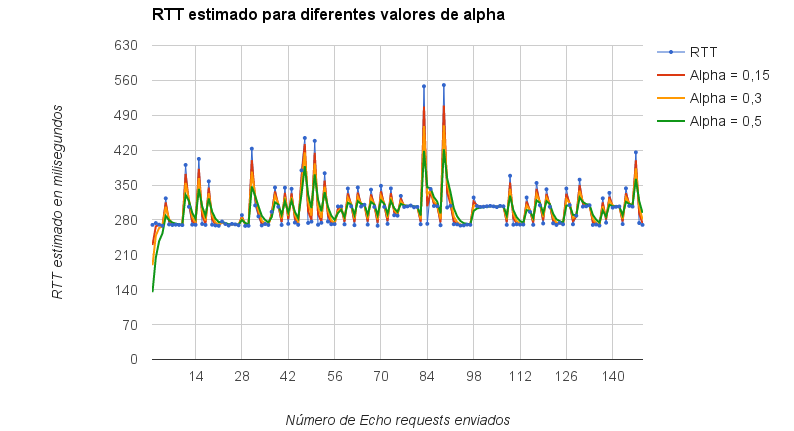
\includegraphics[width=1.5\textwidth]{../Experimentacion/Noruega/ertt.png}
    \caption{RTT estimado por cada muestra de RTT para los diferentes valores de $\alpha$}
  \label{ertt-nor}
\end{changemargin}
\end{figure}

\begin{table}[H]
	\centering
    \begin{tabular}{lllll}
    \hline
    \#Muestras & $\alpha$ & RTT estimado &Prob. estimada perdida paquete & Throughput \\	\hline
    10   &  0.15  &  328.42 ms  &  0.0\%  &  194.8 Kbyte/s  \\
    10   &  0.30  &  335.21 ms  &  0.0\%  &  190.9 Kbyte/s  \\
    10   &  0.50  &  335.69 ms  &  0.0\%  &  190.6 Kbyte/s  \\
    70   &  0.15  &  270.23 ms  &  0.0\%  &  236.8 Kbyte/s  \\
    70   &  0.30  &  272.85 ms  &  0.0\%  &  234.5 Kbyte/s  \\
    70   &  0.50  &  275.58 ms  &  0.0\%  &  229.7 Kbyte/s  \\
    150  &  0.15  &  273.45 ms  &  0.666666666667\%  &  65.4 Kbyte/s  \\
    150  &  0.30  &  281.07 ms  &  0.666666666667\%  &  63.6 Kbyte/s  \\
    150  &  0.50  &  294.13 ms  &  0.666666666667\%  &  60.8 Kbyte/s  \\ \hline
    \end{tabular}
    \caption{Resultado del análisis de las muestras de RTTs para Noruega}
  \label{fig:tabla-ertt-nor}
\end{table}

\subsubsection{Universidad de Tokyo - Japón}

\begin{figure}[H]
\begin{changemargin}{-5cm}{-5cm}
    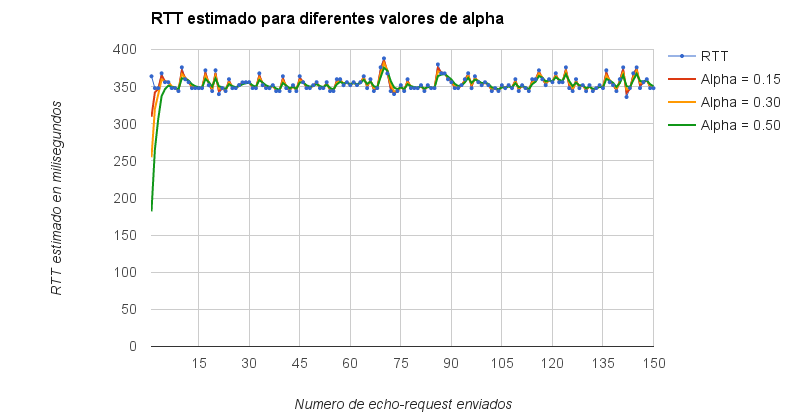
\includegraphics[width=1.5\textwidth]{../Experimentacion/Tokyo/ertt.png}
    \caption{RTT estimado por cada muestra de RTT para los diferentes valores de $\alpha$}
  \label{ertt-tok}
\end{changemargin}
\end{figure}

\begin{table}[H]
	\centering
    \begin{tabular}{lllll}
    \hline
    \#Muestras & $\alpha$ & RTT estimado &Prob. estimada perdida paquete & Throughput \\	\hline
    10   &  0.15  &  307.94 ms  &  0.0\%  &  207.8 Kbyte/s  \\
    10   &  0.30  &  310.33 ms  &  0.0\%  &  206.2 Kbyte/s  \\
    10   &  0.50  &  315.45 ms  &  0.0\%  &  202.8 Kbyte/s  \\
    70   &  0.15  &  295.47 ms  &  5.71428571429\%  &  20.4 Kbyte/s  \\
    70   &  0.30  &  298.96 ms  &  5.71428571429\%  &  20.4 Kbyte/s  \\
    70   &  0.50  &  300.36 ms  &  5.71428571429\%  &  20.3 Kbyte/s  \\
    150  &  0.15  &  299.94 ms  &  4.66666666667\%  &  22.5 Kbyte/s  \\
    150  &  0.30  &  301.54 ms  &  4.66666666667\%  &  22.4 Kbyte/s  \\
    150  &  0.50  &  304.26 ms  &  4.66666666667\%  &  22.2 Kbyte/s  \\ \hline
    \end{tabular}
    \caption{Resultado del análisis de las muestras de RTTs para Rusia}
  \label{fig:tabla-ertt-rus}
\end{table}

\subsubsection{Lomonosov Universidad del estado de Moscú - Rusia}

\begin{figure}[H]
\begin{changemargin}{-5cm}{-5cm}
    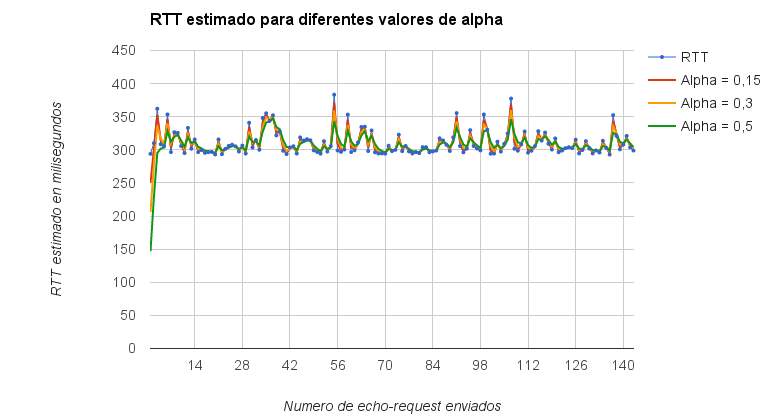
\includegraphics[width=1.5\textwidth]{../Experimentacion/Rusia/ertt.png}
    \caption{RTT estimado por cada muestra de RTT para los diferentes valores de $\alpha$}
  \label{ertt-rus}
\end{changemargin}
\end{figure}

\begin{table}[H]
	\centering
    \begin{tabular}{lllll}
    \hline
    \#Muestras & $\alpha$ & RTT estimado &Prob. estimada perdida paquete & Throughput \\	\hline
    10   &  0.15  &  355.24 ms  &  0.0\%  &  180.1 Kbyte/s  \\
    10   &  0.30  &  355.13 ms  &  0.0\%  &  180.2 Kbyte/s  \\
    10   &  0.50  &  355.14 ms  &  0.0\%  &  180.2 Kbyte/s  \\
    70   &  0.15  &  347.46 ms  &  0.0\%  &  184.1 Kbyte/s  \\
    70   &  0.30  &  347.15 ms  &  0.0\%  &  184.3 Kbyte/s  \\
    70   &  0.50  &  347.15 ms  &  0.0\%  &  184.4 Kbyte/s  \\
    150  &  0.15  &  348.18 ms  &  0.0\%  &  183.8 Kbyte/s  \\
    150  &  0.30  &  348.90 ms  &  0.0\%  &  183.4 Kbyte/s  \\
    150  &  0.50  &  350.55 ms  &  0.0\%  &  182.5 Kbyte/s  \\ \hline
    \end{tabular}
    \caption{Resultado del análisis de las muestras de RTTs para Japon}
  \label{fig:tabla-ertt-tokyo}
\end{table}

